\chapter{Ausführung}

    Dieses Kapitel beschreibt die Vorgehensweise von der ersten manuellen Analyse der Daten bis zu einem funktionierenden neuronalen Netz.
    Außerdem werden verschiedene neuronale Netze miteinander verglichen um die beste Vorgehensweise zur Klassifikation von Geräten zu finden.
    Als Beispielprodukt für die Klassifizierung wurde eine Senseo Kaffeemaschine gewählt, da durch häufige Benutzung viele Daten erhoben werden können. 
    Außerdem wurde eine Mikrowelle als zweite Gerät mit wenigen Daten gewählt um verschiedene Parameter und Kennzahlen zu vergleichen.
    Hierbei soll die Anzahl der Daten sowie die Klassifikation von mehreren Geräten innerhalb eines neuronalen Netzes untersucht werden.

\section{Manuelle Analyse} \label{ManuelleAnalyse}

    \paragraph{Kaffeemaschine}

    Zur manuellen Analyse der Daten wird das in \ref{VisualisierungWebApp} beschriebene Tool verwendet.
    Zunächst werden aussagekräftige Größen wie die Spannung oder die Frequenz der Kaffeemaschine verwendet und mit anderen aktiven Zeiträumen der Kaffeemaschine verglichen.
    Hierbei kann ein spezifischer Verlauf der Spannung erkannt werden.\\ 
    Wie in Abbildung \ref{fig:Spannungsverlauf} zu sehen ist, ist die Kurve zu Beginn stark fallend und verbleibt dann eine gewissen Zeit auf diesem Tief. 
    Nach einem länger steigenden Abschnitt fällt die Kurve wieder bis der Zubereitungsvorgang beendet wurde und die Spannung wieder steigt.\\
    

    Diesem Verlauf können nach mehreren Beobachtungen bestimmte Vorgänge einer Kaffeezubereitung zugeordnet werden.
    Durch die Erwärmung des Brühwassers, beim Einschalten der Kaffeemaschine, kann ein erstes Fallen der Kurve beobachtet werden.
    Da dabei viel Energie benötigt um das Wasser zu erhitzen, steigt der Stromverbrauch der Kaffeemaschine stark an; somit fällt die Netzspannung stark ab.
    Die Netzspannung bleibt solange auf einem gewissen Tiefpunkt mit minmaler Netzschwankung bis das Wasser erwärmt wurde und ein weiterer manueller Schritt zum Fortfahren des Prozesses notwendig ist.\\
    

    Nach manueller Wahl der Tassengröße wird der Brühvorgang gestartet. 
    Dabei wird das erhitzte Wasser mit einem gewissen Druck durch einen Kaffeepad gepresst. 
    Da dieser Druck bei der Senseo Kaffeemaschine durch eine elektronische Pumpe erzeugt wird, sinkt demnach die Netzspannung wieder ab bis der komplette Vorgang beendet ist.
    Somit kann die zweite Tiefpunktphase dem "`Pressvorgang"' der Kaffeemaschine zugeordnet werden.\\
    \newline
    
    \begin{figure}[H]
        \centering
        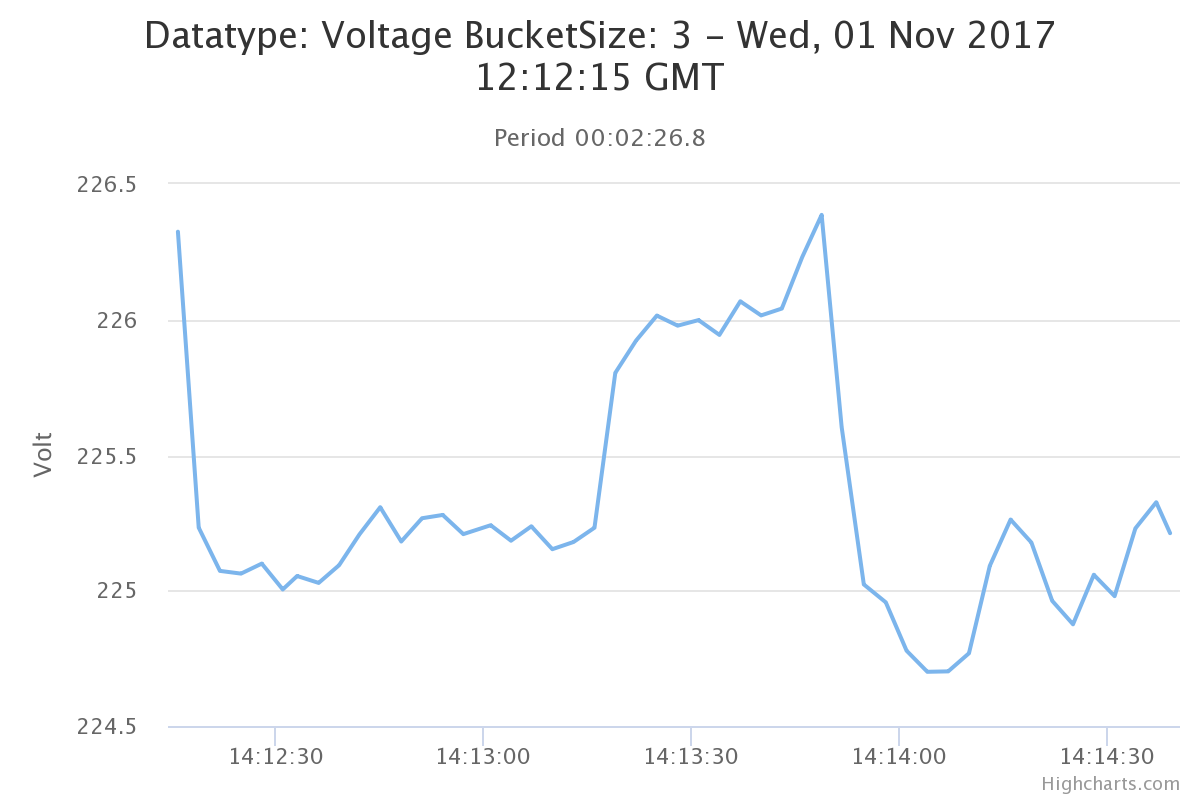
\includegraphics[width=0.8\textwidth]{SpannungsverlaufSenseo1}
        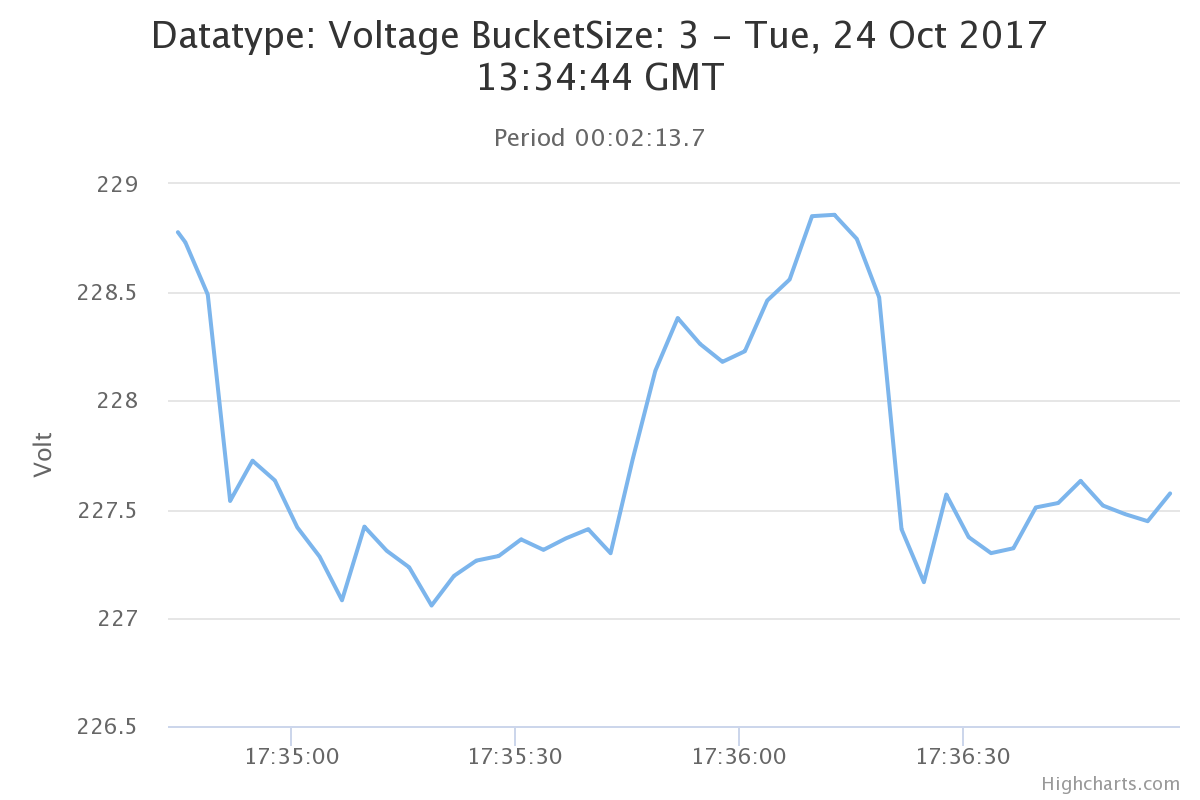
\includegraphics[width=0.8\textwidth]{SpannungsverlaufSenseo2}
        \caption{Spannungsverlauf der Senseo Kaffeemaschine mit einer Klasse von je 3 Datenpunkten zu 2 verschiedenen Zeitpunkten}
        \label{fig:SpannungsverlaufSenseo}
    \end{figure}

    \paragraph{Mikrowelle}

    Bei der manuellen Analyse der Mikrowelle können bei dem Spannungs- oder Frequenzverlauf keine hervorstechenden Merkmale oder Gemeinsamkeiten erkannt werden.
    Somit wird die Mikrowelle demnach einen anderen Einfluss auf die Netzaktivität ausüben.
    Wie bei dem Vergleich der verschiedenen harmonischen Oberwellen zu sehen ist (siehe Abbildung \ref{fig:3OberwelleMikrowelle}), besteht eine große Ähnlichkeit der Kurven der dritten harmonischen Welle.\\

    \begin{figure}[H]
        \centering
        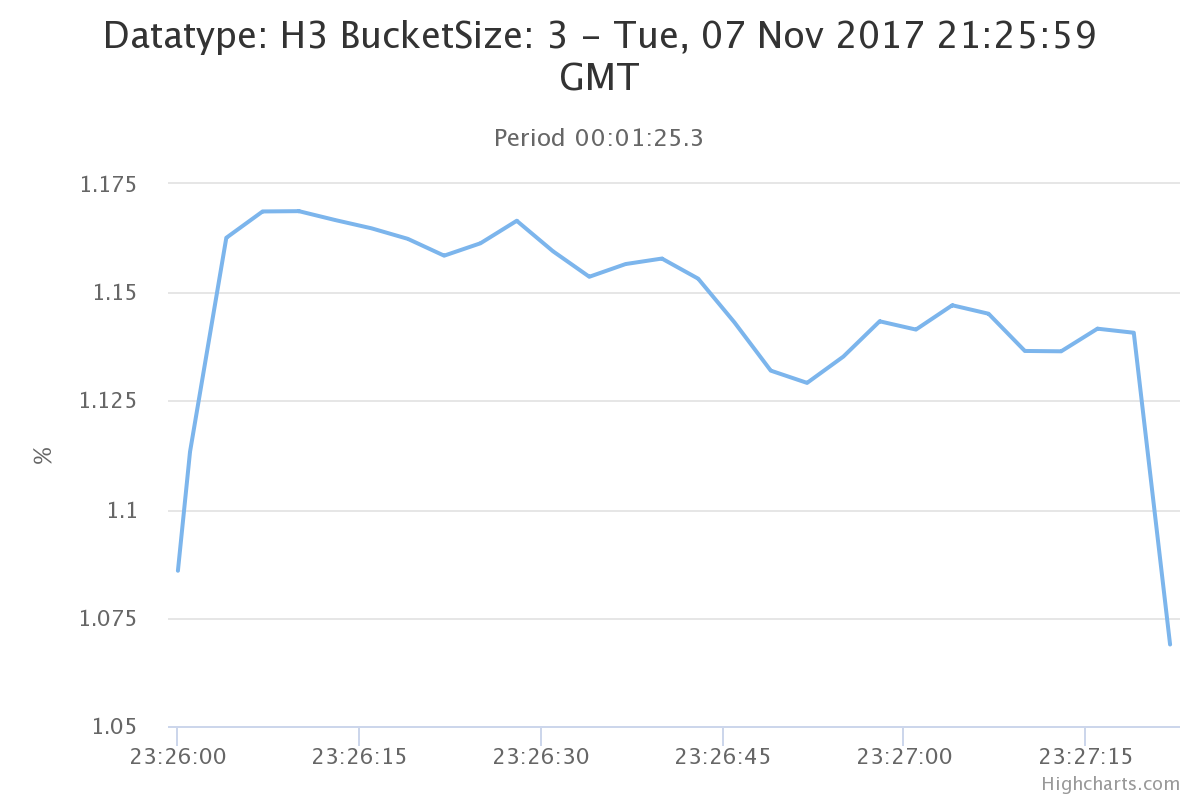
\includegraphics[width=0.8\textwidth]{3OberwelleMikrowelle1}
        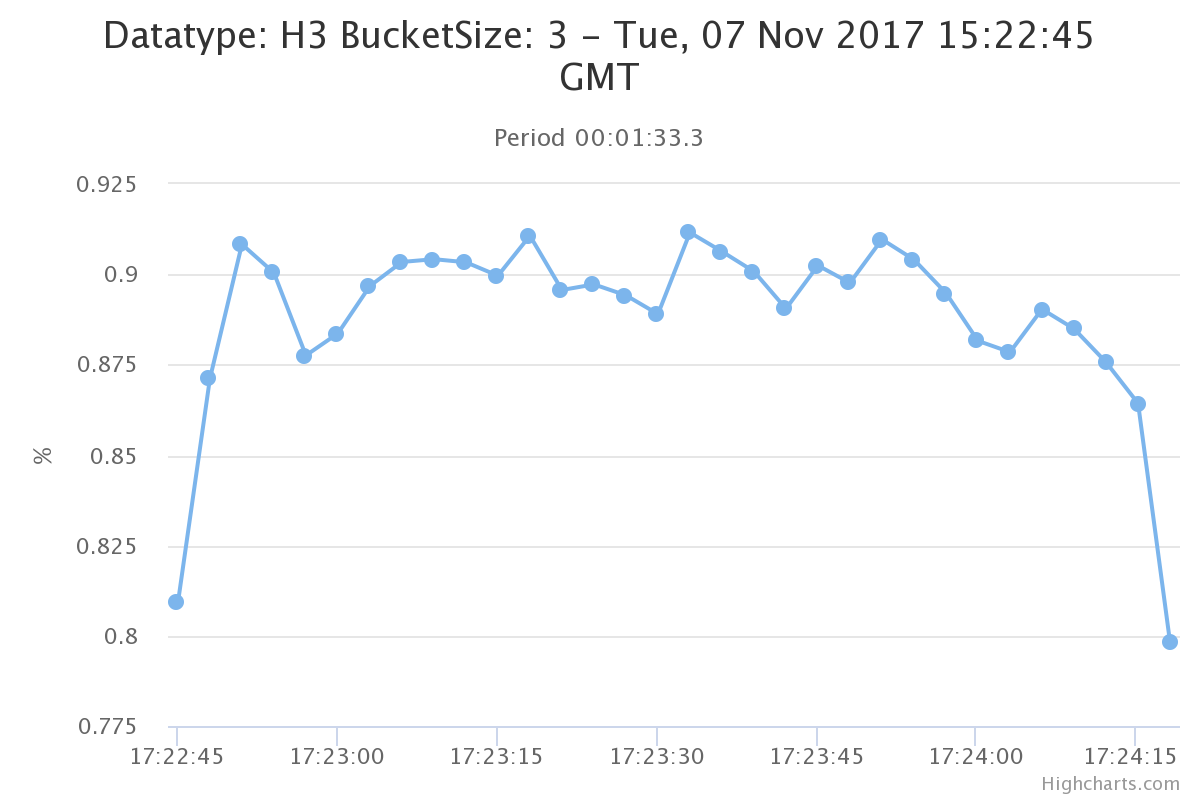
\includegraphics[width=0.8\textwidth]{3OberwelleMikrowelle2}
        \caption{Verlauf der 3. harmonischen Oberwelle einer Mikrowelle mit einer Klasse von je 3 Datenpunkten zu 2 verschiedenen Zeitpunkten}
        \label{fig:3OberwelleMikrowelle}
    \end{figure}

    \noindent
    Wie dieser Abschnitt zeigt, können schon mit bloßem Auge bestimmte Auswirkungen der verschiedenen Geräte erkannt werden.
    Auch wenn einige Störungen auftreten und den Verlauf verfälschen, sollte es dennoch möglich sein diese Geräte herauszufiltern.
    \newline
    
    Weiterführend wird dieser Prozess automatisiert und verbessert um auch trotz großer Störungen, Geräte präzise klassifizieren zu können. 

\section{Vorbereiten der Daten}\label{VorbereitenDerDaten}
    Um die Klassifizierung der Geräte auf neuronalen Netzen abzubilden, müssen die vorhandenen Daten in ein geeignetes Format transformiert werden.
    Um die verschiedenen Formen der Transformation durchzuführen müssen bestimmte Voraussetzungen beachtet werden.
    Die Implementierung zu diesen Kapitel lässt sich in \footnote{\url{https://github.com/schrodit/wesense-ml/blob/master/data/data_manager.py}} finden.\\
    
    \noindent
    Bei konventionellen neuronalen Netzen werden Eigenschaften Objekten zugewiesen, wobei alle Objekte mit denselben Eigenschaften beschrieben werden.
    Ein Beispiel dafür sind Tiere, bei denen anhand von Reproduktion oder Atmung, in Säugetiere, Vögel, Reptilien, etc. eingeteilt werden. 
    So können speziellen Tieren, wie einem Hund, eine dieser Klassen zugewiesen werden.
    Allen klassifizierten Tieren werden hierbei dieselben Eigenschaftsklassen mit unterschiedlichen Werten zugewiesen.
    Das heißt, dass einem Hund oder einer Taube die Anzahl der Beine und die Reproduktion zugewiesen werden, jedoch mit jeweils unterschiedlichen Werten.\\
    %besser beschreiben 4 Füße
    
    Durch die in Kapitel \ref{Messdaten} beschriebene Erhebung der Daten werden die Stromdaten in einem bestimmten Format von der API bereitgestellt.
    Es werden 2 verschiedene Listen zurückgegeben wobei eine die reinen Messdaten enthält und die andere die Labels für diese Daten.\\
    Die reinen Messdaten werden zusammengetragen, indem zu den gelabelten Zeiträumen jeweils alle sekündlich gemessenen Werte des Stromnetzes als Matrix eingefügt werden.
    \newline

    \noindent
    Zusätzlich zu den manuell klassifizierten Daten werden noch zufällig ausgewählte Zeitabschnitte hinzugefügt um die Möglichkeit "`kein Gerät war aktiv"' abzubilden.
    Diese Abschnitte werden gewählt, indem willkürlich Daten aus der Datenbank abgerufen werden bei denen mit großer Wahrscheinlich kein zu klassifizierendes Gerät aktiv war.
    Als einer dieser Zeiträume könnte zum Beispiel von 00:00 bis 5:00 Uhr gewählt werden, da zu dieser Zeit mit hoher Wahrscheinlichkeit kein Gerät aktiv war.
    \newline

    \noindent
    Somit ergibt sich eine dreidimensionale Matrix, welche in der ersten Dimension die Zeiträume abbildet, in der zweiten Dimension die sekündliche Zeitreihe und in der dritten die vorhandenen physikalischen Größen.

    \begin{lstlisting}[language=Python, caption={Datenstruktur der gelabelten Messdaten, die von der API bereit gestellt wird},label=lst:DatenstrukturGelabelteMessdaten]

[
    [
        [u, f, h3, h5, h7, h9, h11, h13, h15],
        [u, f, h3, h5, h7, h9, h11, h13, h15],
        [u, f, h3, h5, h7, h9, h11, h13, h15],
        ...
    ]
]
    \end{lstlisting}

    Da neuronale Netze feste Eingabegrößen benötigen, werden die Daten in Batches aufgeteilt.
    Batches bedeutet, dass die Zeitreihe in gleich große Abschnitte aufgeteilt wird.
    Dementsprechend wird die Matrix \( A[m, n, 9] \), zu einer Matrix mit einheitlicher Größe transformiert, sodass die entstehende Matrix zum Beispiel die Form \( B[m, 20, 9] \) annimmt.
    \newline

    \noindent
    Um diese neue Matrix zu erhalten wird folgender Algorithmus auf die alte Matrix angewandt:

    \begin{algorithm}\label{alg:BatchGenerierung}
        \caption{Batch Generierung}
        \begin{algorithmic}[1]
        \Function{GeneriereBatches}{$A,b$}
        \State\Comment{A - float[][][], b - int (Batchgröße)}
            \State ${B} = Array[][][]$
            \For{$i = 0$ to $length(A)$}
                \For{$j = 0$ to $length(A[i]) - b$}
                    \State $start = j$
                    \State $end = j + b$ 
                    \State $I_b = length(B) + 1$
                    \State $B[I_b] = A[i][start : end]$
                \EndFor
            \EndFor
            \State return $B$
        \EndFunction
        \end{algorithmic}
    \end{algorithm}

\section{Neuronales Netz}
    Wie Abschnitt \ref{ManuelleAnalyse} zeigt, ist es möglich, mit herkömmlichen manuellen Methoden verschiedene Geräte innerhalb eines Verlaufs zu klassifizieren.
    Somit sollte dies auch mit maschinellem Lernen möglich sein.
    \newline

    \noindent
    Um die Geräte maschinell zu klassifizieren, werden drei verschiedene "`neuronale Netzmodelle"' erstellt und miteinander verglichen.
    Die drei Modelle beinhalten ein "`Recurrent Neural Network(RNN) "', ein "`Convolutional Neural Network(CNN)"' sowie eine Mischung aus diesen Ansätzen. 
    Bei allen Modellen wurde als Gradientenverfahren die Adam-Optimierung gewählt, da diese bei mehr Rechenaufwand bessere Ergebnisse erzielt.    

    \subsubsection{CNN}
    Grundlegend besteht das \ac{CNN} aus einem "`Input Layer"', drei "`Convolutional Layers"', einem "`Dropout Layer"' sowie einem "`Output Layer"'(vgl. \footnote{\url{https://github.com/schrodit/wesense-ml/blob/master/classification/cnn_classification.py}}).
    \newline

    \noindent
    Der "`Input Layer"' ist der Eingang zum neuronalen Netz, welcher die Rohdaten annimmt und an das eigentliche Netz weiterleitet. 
    Es ist ein weiteres "`Convolutional Layer"' und nimmt einen Tensor (Matrix innerhalb eines neuronalen Netzes) als Eingabe, welcher an die Batchgröße angepasst ist.
    Dementsprechend hat der Eingabetensor die Form \( A[m, b, 9] \), mit m: Trainingsdatengröße und b: Batchgröße.
    \newline

    \noindent
    Die Eingabe wird dann weitergeleitet an die drei "`Convolutional Layers"', welche mit unterschiedlicher "`Hidden Layer"'-Größe initialisiert werden.
    Die "`Hidden Layer"' werden größer je näher sie topologisch an dem "`Output Layer"' liegen.
    \newline

    \noindent
    Der "`Dropout Layer"' wird eingefügt um die Tensordimension zu verkleinern und somit das Ergebnis zu generalisieren und "`overfitting"' zu vermeiden.
    \newline

    \noindent
    Der "`Output Layer"' wandelt nun die Erkenntnisse der vorherigen Schichten in ein lesbares Format um. 
    Hierbei wird ein "`Dense Layer"' verwendet, welcher ein eindimensionaler Tensor mit einem Feld pro klassifizierbaren Objekt ist und die Softmax-Funktion als Aktivierungsfunktion beinhaltet.
    Dieser eindimensionale Tensor repräsentiert pro Feld die Ausgabe der zu klassifizierenden Geräte.     
    
    \begin{figure}[H]
        \centering
        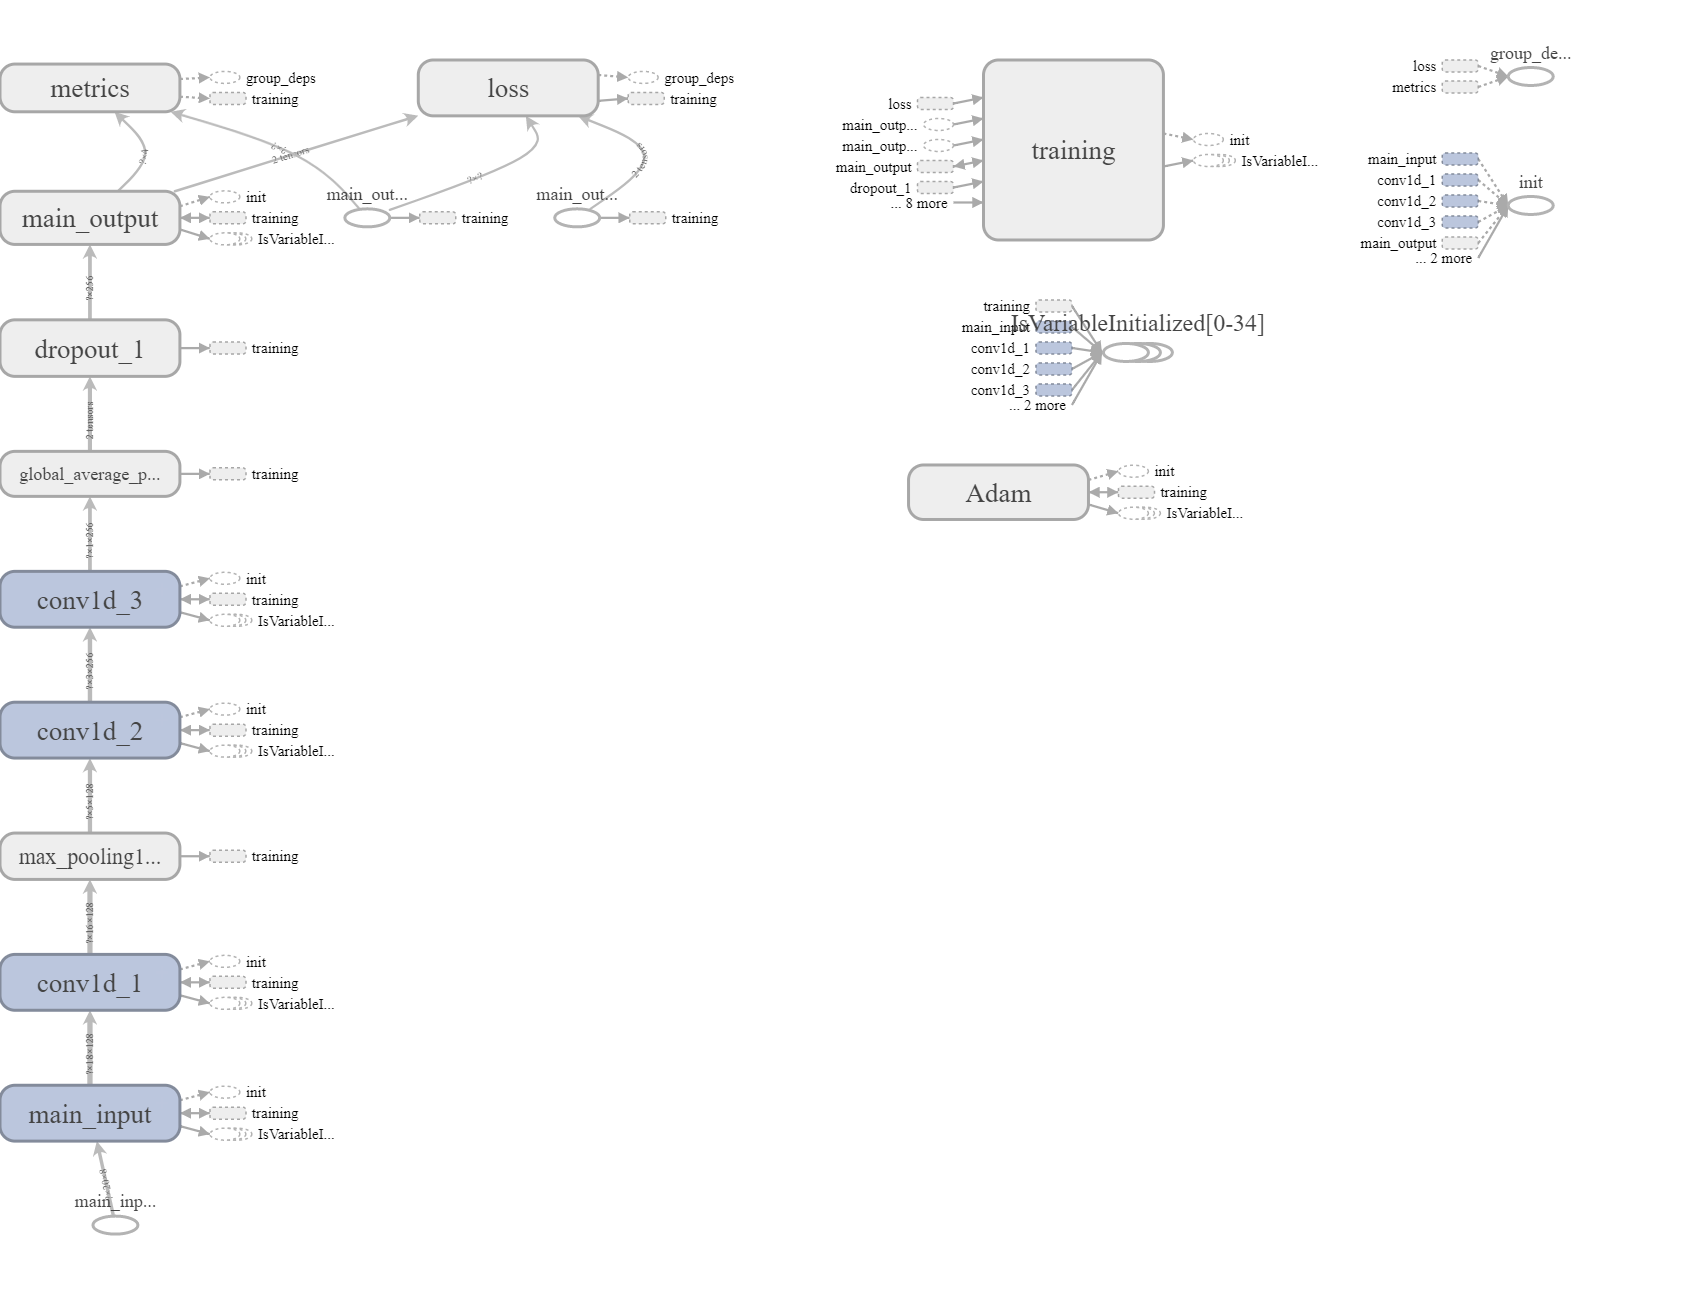
\includegraphics[width=\textwidth]{CNN_Model}
        \caption{Convolutional Neural Network \protect\cite{Tensorboard}}
        \label{fig:CNN_MODEL}
    \end{figure}

    \subsubsection{RNN}
    Das "`Recurrent Neural Network(RNN) "'- Model besteht aus einem "`Input Layer"', zwei darauffolgenden "`LSTM(Long short-term memory) Layer"' und einem "`Ouput Layer"' (vgl. \footnote{\url{https://github.com/schrodit/wesense-ml/blob/master/classification/rnn_classification_keras.py}}).\\
    \noindent
    Der "`Input Layer"' ist ein weiteres "`LSTM Layer"', welcher denselben Eingabetensor annimmt wie das CNN-Model.\\
    \noindent
    Es folgen zwei weitere "`LSTM Layer"' einer "`Hidden Layer"'-Größe von 64 Neuronen pro Schicht.
    Dieselbe Größe wird auch im Eingabe-"`LSTM Layer"' verwendet.
    \newline

    \noindent
    Der "`Output Layer"' ist, wie beim \ac{CNN}-Model, ein "`Dense Layer"', der aus der Berechnung des Netzes eine verwertbare Ausgabe erzeugt.

    \begin{figure}[H]
        \centering
        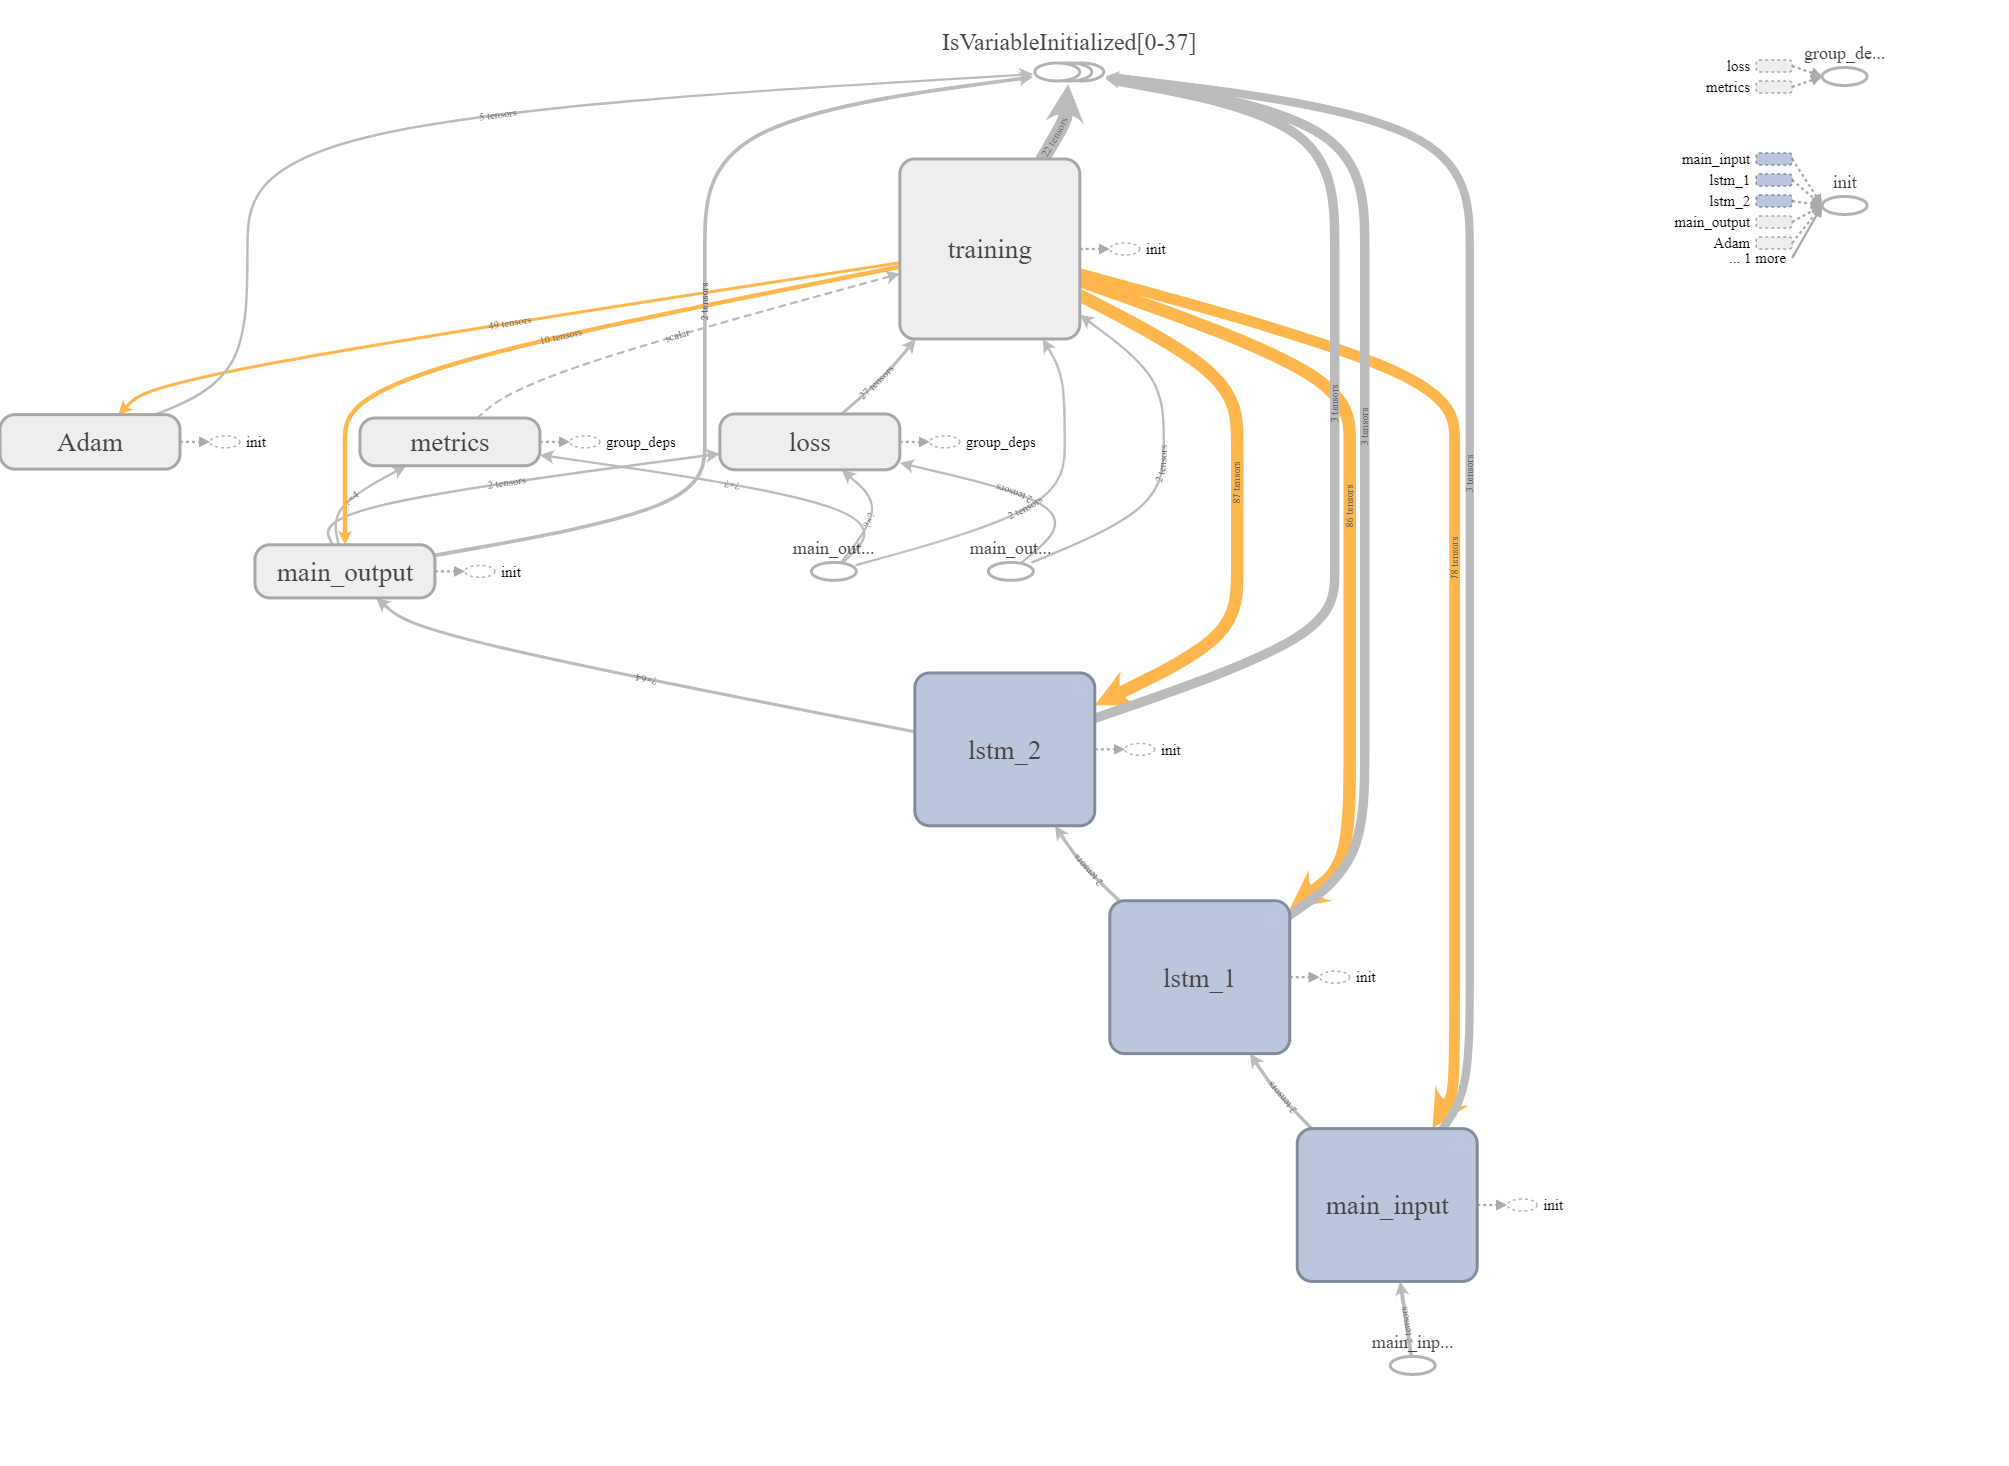
\includegraphics[width=\textwidth]{RNN_Model}
        \caption{Recurrent Neural Network \protect\cite{Tensorboard}}
        \label{fig:RNN_MODEL}
    \end{figure}

    \subsubsection{Mixed - CNN und RNN}
    Das dritte zu testende Model beinhaltet eine Mischung aus den zwei bisherigen Netzen. 
    Dies soll zeigen, ob verschiedene Eigenschaften, von neuronalen Netzen, positive oder negative Auswirkungen auf das Training und die Genauigkeit des Models haben.
    \newline

    \noindent
    Da dieses Model eine Mischform aus \ac{CNN} und \ac{RNN} ist, besteht dieses Model aus zwei "`Convolutional Layers"', welche die Eingabe und eine Vorprozessierung zum Generalisieren der Eingabe darstellt (vgl. \footnote{\url{https://github.com/schrodit/wesense-ml/blob/master/classification/mix_classification.py}}).
    Auf diese beiden Schichten folgen zwei rekurrente "`LSTM Layer"' und dasselbe "`Output Layer"' wie bei beiden anderen Modellen.
    Die \ac{RNN}-Schichten sollen das Vorprozessierte verarbeiten um mögliche Muster in der Zeitserie zu erkennen.     

    \begin{figure}[H]
        \centering
        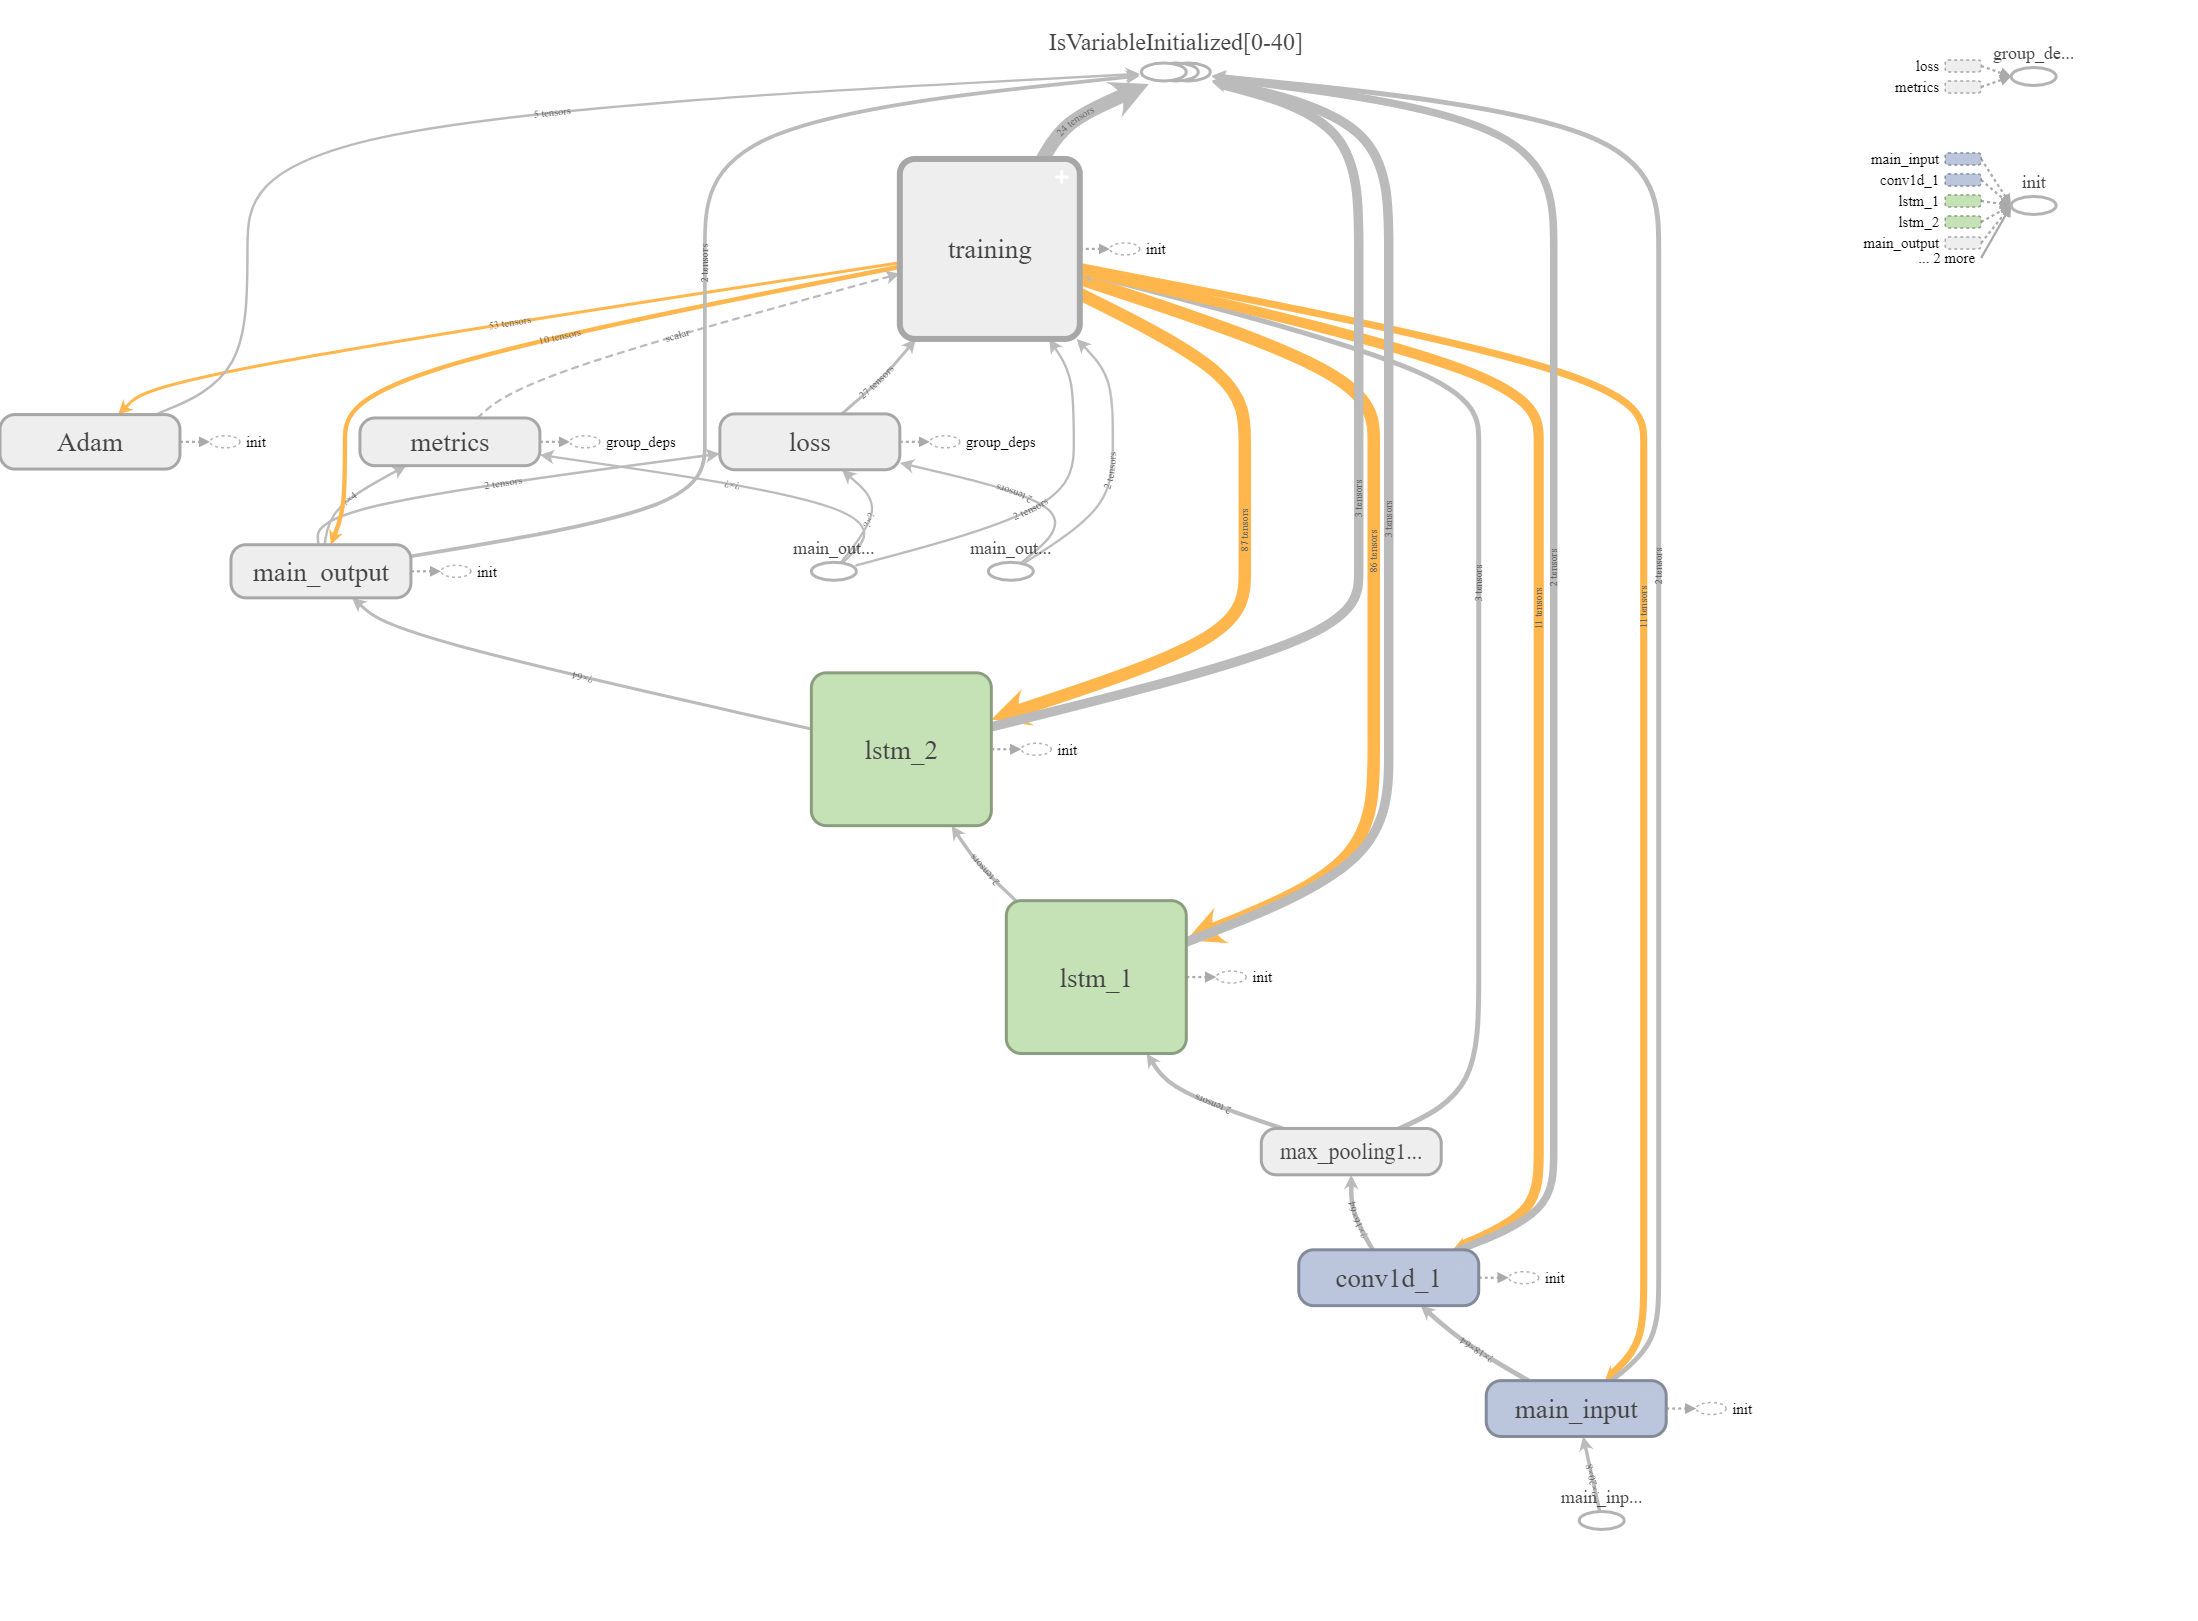
\includegraphics[width=\textwidth]{MIX_Model}
        \caption{\ac{CNN} mit \ac{RNN} \protect\cite{Tensorboard}}
        \label{fig:MIX_MODEL}
    \end{figure}

    Die in diesem Abschnitt dargestellten Modelle stellen den grundlegenden Aufbau der neuronalen Netze dar.
    Diese beinhalten jedoch keinerlei Wissen und können somit noch nicht zum Klassifizieren verwendet werden.    


\section{Trainingsprozess}
    Um die drei verschiedene Modelle anwenden zu können, muss diesen Wissen beigebracht werden.
    Dies geschieht durch Trainieren, mit den in Abschnitt \ref{VorbereitenDerDaten} vorbereiteten Daten(vgl. Abschnitt \ref{KlassifikationDerMessdaten}).
    Damit die Modelle bestmögliche Ergebnisse erzielen, wird der Trainingsprozess mit verschiedenen Trainingsparametern sowie verschiedenen Daten durchlaufen.
    Die Trainingsparameter beinhalten die Batchgöße, die Lernrate, die Trainingsepochen, die Anzahl der zusätzlich gewählten Zeiträume sowie die genutzten physikalischen Größen.
    \newline

    \noindent
    Die Trainingsparameter aller Netze werden zunächst mit Standardparametern versehen.
    \newline
    \noindent
    Diese Standardparametern werden wie folgt festgelegt:\\
    \noindent
    Lernrate = 0.001\\
    \noindent
    Datentypen = ['u', 'h3', 'h5', 'h7', 'h9', 'h11', 'h13', 'h15']\\
    \noindent
    Batchgröße = 20\\
    \noindent
    Epochen = 30\\

    \noindent
    Um die Auswirkung einzelner Parameter auf das Trainingsergebnis sehen zu können wird jeweils ein Parameter verändert um verschiedene Werte dieses Parameters miteinander verglichen.
    \newline
    \noindent
    Als Maßstab der Beeinflussung eines Parameters auf das Ergebnis eines Models wird die Genauigkeit sowie die Validierungsgenauigkeit in Prozent gewählt.
    Diese Werte werden nach dem Training eines Models, anhand von Test- bzw. Validierungsdaten, errechnet (vgl. Abschnitt \ref{Lernprozess}). 
    Somit kann mit der Genauigkeit das Erlernen der Trainingsdaten überprüft werden, sowie mit der Validierungsgenauigkeit Over- bzw. Underfitting des Models nachgewiesen werden.
    \newline

    \noindent
    Nach einigen Trainingsversuchen (vgl. Tabelle \ref{tabl:ErgebnisAbleitung}) mit den Rohdaten wurde festgestellt, dass mit diesen Daten keine aussagekräftigen Ergebnisse erzielt werden können.
    Als Lösung dieses Problems werden nach einigen Versuchen zwei Verfahren gewählt mit denen die Rohdaten transformiert werden. \\
    \noindent
    Es wird eine Normalisierung der Daten in Werte zwischen 0-1 durchgeführt, sodass größere Werte wie die Spannung, welche bei ca. 230V liegt, keinen höheren Einfluss auf das Ergebnis haben kann als die Frequenz.\\
    \noindent
    Zusätzlich werden die Ableitungen über alle Werte der Rohdaten berechnet.
    Dies führt dazu, dass vom neuronalen Netz der Verlauf der Kurve berücksichtigt wird und nicht die reinen Rohwerte, welche je nach Netzwerk und aktueller Netzaktivität stark abweichen können, nicht berücksichtigt.

    \begin{table}[H]
        \centering
        \begin{tabular}{|c|c|c|c|}
            \hline
            Model & Genauigkeit & Validierungsgenauigkeit \\
            \hline
            CNN & 85,69\% & 85,78\% \\
            \hline
            RNN & 87,99\% & 86,68\% \\
            \hline
            MIX & 48,13\% & 48,42\% \\
            \hline
        \end{tabular}
        \caption{Ergebnis: Ableitung}
        \label{tabl:ErgebnisAbleitung}
    \end{table}

    \section{Auswertungsalgorithmus}\label{Auswertungsalgorithmus}
        Nach der Klassifikation der Batches mit einem der neuronalen Netze, sind für diese klassifizierten Batches mit n Datenpunkten für jeden Punkt n Klassifizierungen vorhandenen(vgl. Algorithmus \ref{alg:BatchGenerierung}).
        Somit muss diese Klassifikation ausgewertet werden, um genau sagen zu können, zu welchen Datenpunkten(Zeitpunkten) welche am wahrscheinlichsten Geräte aktiv waren.
        Hierzu wird der Algorithmus in \ref{alg:Ergbnisauswertung} verwendet, welcher die Treffer sowie die genaue Wahrscheinlichkeit pro Klasse zu einem bestimmten Zeitpunkt berücksichtigt. 
        Dieser Algorithmus bestimmt die Anzahl der Gewinnerklassen (Klasse mit der höchsten Wahrscheinlichkeit) aller Batches in denen der bestimmte Datenpunkt vorhanden ist, und bestimmt nun aus dieser Anzahl wiederum die Gewinnerklasse (Klasse mit den meisten Treffern).
        Außerdem wird die Wahrscheinlichkeit aller Klassen in allen Batches des Datenpunktes summiert und die Gewinnerklasse bestimmt.
        Somit erhält man zwei verschiedene Gewinnerklassen, welche miteinander verglichen werden um die endgültige Gewinnerklasse zu bestimmen.

        Der Vorteil dieses Verfahrens ist die Berücksichtigung aller Klassifikationen sowie deren Einzelwahrscheinlichkeit, sodass sich eine genauere Klassifizierung ergibt, wie Abbildung \ref{fig:CNN_RawClassification} zeigt.
        \begin{algorithm}\label{alg:Ergbnisauswertung}
            \caption{Ergbnisauswertung}
            \begin{algorithmic}[1]
            \Function{EvaluatePrediction}{$P,b$}
                \State \Comment{P - int[][] (Ergebnis eines neuronalen Netzes), b - int (Batchgröße)}
                \State
                \State ${A} = int[ ]$
                \For{$i = 0$ to $length(P)$}
                    \State
                    \State // Hit-Punkte aller Klassen für einen Zeitpunkt
                    \State $ClassesHit = int[ ]$
                    \State // Wahrscheinlichkeit aller Klassen für einen Zeitpunkt
                    \State $ClassesPerc = float[ ]$
                    \State
                    \If{$i < b$}
                        \State $start = 0$
                        \State $end = i$
                    \Else
                        \State $start = i - b$
                        \State $end = i$
                    \EndIf
                    \State
                    \For{$d = start$ to $end$}
                        \State $maxClassIndex = argmax(pred[d])$
                        \State $ClassesHit[maxClassIndex]++$

                        \For{$w = 0$ to $pred[d]$}
                            \State $ClassesPerc[w] = ClassesPerc[w] + pred[d][w]$
                        \EndFor
                    \EndFor
                    \State
                    \State $A.append(EvaluateClasses(ClassesHit, ClassesPerc))$
                    \State
                \EndFor
                \State return $A$
            \EndFunction
            \end{algorithmic}
        \end{algorithm}
        \begin{algorithm}
            \caption{Ergebnis-Klassen-Auswertung}
            \begin{algorithmic}[1]
            \Function{EvaluateClasses}{$ClassesHit, ClassesPerc$}
                \State \Comment{ClassesHit - int[], ClassesPerc - float[]}
                \State
                \State $MaxHitClass = argmax(ClassesHit)$
                \State $MaxPercClass = argmax(ClassesPerc)$
                \State
                \If{$MaxHitClass == MaxPercClass$}
                    \State return $MaxHitClass$
                \Else
                    \State
                    \State $MaxHitClassPerc = ClassesHit[MaxHitClass] / Sum(ClassesHit) $
                    \State $MaxPercClassPerc = MaxPercClass[MaxHitClass] / Sum(ClassesPerc) $
                    \State
                    \If{$$MaxHitClassPerc < MaxPercClassPerc$$}
                        \State return $MaxPercClass$
                    \Else
                        \State return $MaxPercClass$
                    \EndIf
                \EndIf
            \EndFunction
            \end{algorithmic}
        \end{algorithm}